\documentclass{article}%
\usepackage[T1]{fontenc}%
\usepackage[utf8]{inputenc}%
\usepackage{lmodern}%
\usepackage{textcomp}%
\usepackage{lastpage}%
\usepackage[head=40pt,margin=0.5in,bottom=0.6in]{geometry}%
\usepackage{graphicx}%
%
\title{\textbf{Ortega Díaz: El gobierno de EE UU debería aprehender a Nicolás Maduro}}%
\author{El Nacional Web}%
\date{26/09/2018}%
%
\begin{document}%
\normalsize%
\maketitle%
\textbf{URL: }%
http://www.el{-}nacional.com/noticias/politica/ortega{-}diaz{-}gobierno{-}deberia{-}aprehender{-}nicolas{-}maduro\_253323\newline%
%
\textbf{Periodico: }%
EN, %
ID: %
253323, %
Seccion: %
Política\newline%
%
\textbf{Palabras Claves: }%
NO\_TIENE\newline%
%
\textbf{Derecho: }%
1.10%
, Otros Derechos: %
NO\_TIENE%
, Sub Derechos: %
1.10.2%
\newline%
%
\textbf{EP: }%
NO\newline%
\newline%
%
\textbf{\textit{El presidente de Venezuela llegó este miércoles a Estados Unidos para participar en la Asamblea General de la ONU}}%
\newline%
\newline%
%
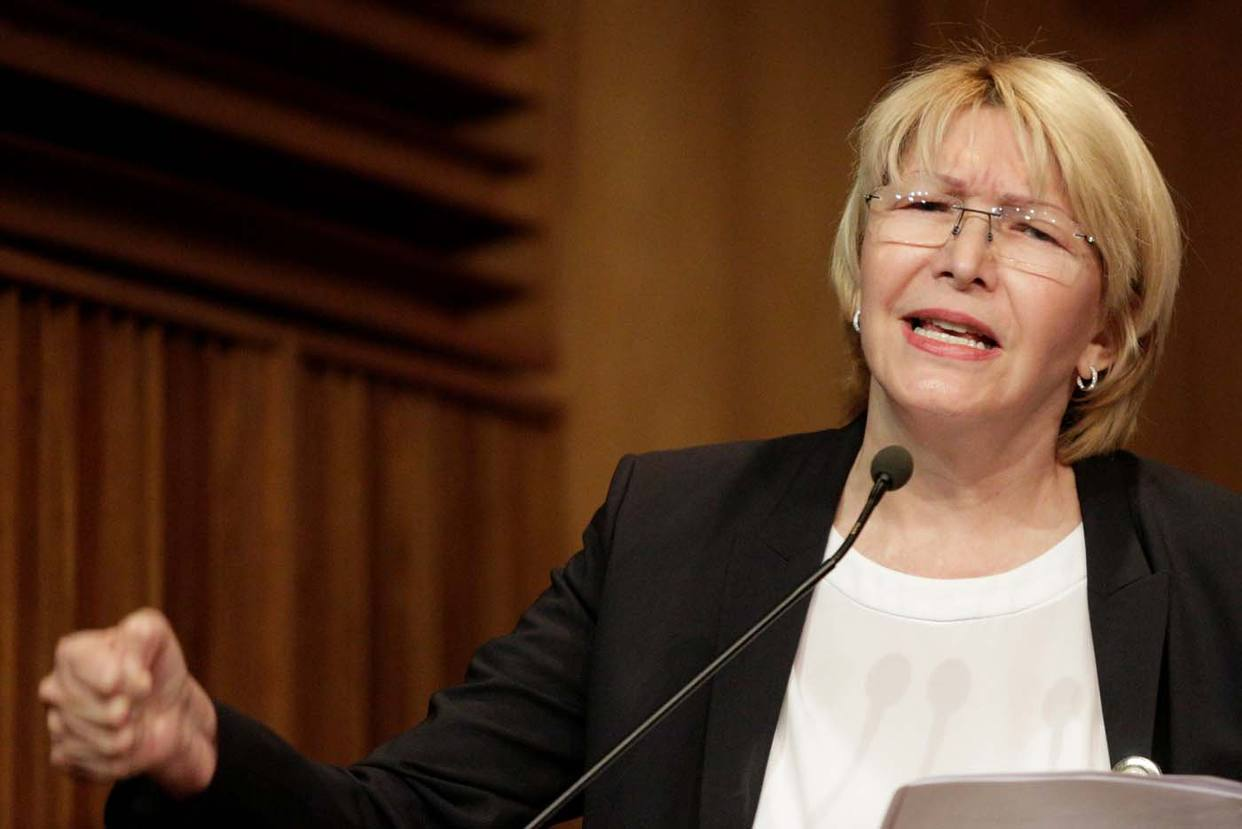
\includegraphics[width=300px]{257.jpg}%
\newline%
%
Luisa Ortega Díaz, fiscal en el exilio, dijo este miércoles que el gobierno de Estados Unidos debería aprehender al presidente Nicolás Maduro luego de que éste anunciara su llegada al país norteamericano para participar en la Asamblea General de la Organización de las Naciones Unidas.%
\newline%
%
La fiscal indicó~"el gobierno de Estados Unidos debe aprovechar que Maduro está en territorio norteamericano para aprehenderlo luego de todas las sentencias y señalamientos que se le han hecho, como crimen organizado, terrorismo, narcotráfico, corrupción y genocidio" durante una entrevista para~W Radio Colombia.%
\newline%
%
Ortega Díaz aseguró que si el presidente de Venezuela se reúne con el mandatario de EE UU, Donald Trump, Maduro se burlará de este país y alegará que los apoya en su modelo de gobierno y decisiones. Luisa dijo esto luego de que se anunciara que Maduro anunció que se reuniría con Trump, quien negó dicho encuentro.%
\newline%
%
Durante la entrevista, rechazó que se realizara cualquier acción belicista en Venezuela por ser no deseables. "Debe retomarse de nuevo la calle para rechazar a Maduro y reclamar sus derechos. Los militares no apoyan al presidente".%
\newline%
%
A pesar de no apoyar las intervenciones, Luisa aseguró que quisiera volver a Venezuela y que se restituya el orden en el país. "Yo nunca quise irme pero fui perseguida por hacer mi trabajo".%
\newline%
%
Puede escuchar las entrevista~aquí%
\newline%
%
\end{document}